\documentclass[14pt]{extarticle}
\usepackage[left=20mm, top=15mm, right=20mm, bottom=15mm, nohead, footskip=10mm]{geometry}
\usepackage[T2A]{fontenc}
\usepackage[russian]{babel}
\usepackage[utf8]{inputenc}
\usepackage{graphicx}
\usepackage{amsmath}
\usepackage{listings}
\usepackage{minted}
\begin{document}

\begin{center}
\hfill \break
\large{Министерство науки и высшего образования Российской федерации}\\
\footnotesize{ФЕДЕРАЛЬНОЕ ГОСУДАРСТВЕННОЕ БЮДЖЕТНОЕ ОБРАЗОВАТЕЛЬНОЕ УЧРЕЖДЕНИЕ}\\
\footnotesize{ВЫСШЕГО ПРОФЕССИОНАЛЬНОГО ОБРАЗОВАНИЯ}\\
\small{\textbf{«АЛТАЙСКИЙ ГОСУДАРСТВЕННЫЙ УНИВЕРСИТЕТ»}}\\
\hfill \break
\normalsize{Институт цифровых технологий, электроники и физики}\\
 \hfill \break
\normalsize{Кафедра вычислительной техники и электроники}\\
\hfill\break
\hfill \break
\hfill \break
\hfill \break
\large{Курс <<Математическое моделирование>>\\ Отчет по лабораторной работе №2\\ <<Модель Ва-тор>>}\\
\end{center}
\hfill \break
\hfill \break
\hfill \break
\hfill \break
\hfill \break

\normalsize{
  \begin{flushright}
    \begin{tabular}{rcr}
      & Выполнил: & студент 585гр.\\\\
      & Роженцев А.К. &\underline{\hspace{3cm}}\\\\
      & Проверил: ст.пр.\\\\
      & Уланов П.Н. & \underline{\hspace{3cm}}
    \end{tabular}
  \end{flushright}
}
\hfill \break
\hfill \break
\hfill \break
\hfill \break
\hfill \break
\begin{center} Барнаул 2020 \end{center}
\thispagestyle{empty}
\newpage
\section{Цель работы}
Написать программу, реализующую модель Ва-Тор, с возможностью сохранения в файл количества рыб и акул на каждом шаге. Выполнить исследование поведения популяций рыб и акул.

\section{Описание модели}
Рыбы: Начальное количество рыб и акул помещается случайным образом в
узлы прямоугольной сетки.Всем рыбам и акулам приписывается случайный
возраст. На очередном временном шаге рассматривается по очереди каждая
рыба. Определяется число ближайших незанятых соседних узлов и рыба
передвигается в один из незанятых узлов случайным образом. Если все
узлы заняты, рыба не перемещается.
Акулы: На очередном временном шаге рассматривается по очереди каждая акула. Если все ближайшие к акуле соседние узлы свободны, она перемещается в один из них случайным образом. Если хоть в одном из них
находится рыба, акула перемещается в такой узел случайным образом и
съедает рыбу. Если за Na шагов акула ничего не съедает, то она погибает. Если акула выживает в течение Ma шагов, у нее появляется потомок.
Новая акула помещается в предыдущую позицию родителя.


\newpage
\section{Программа}


\begin{figure}[!h]
  \centering
  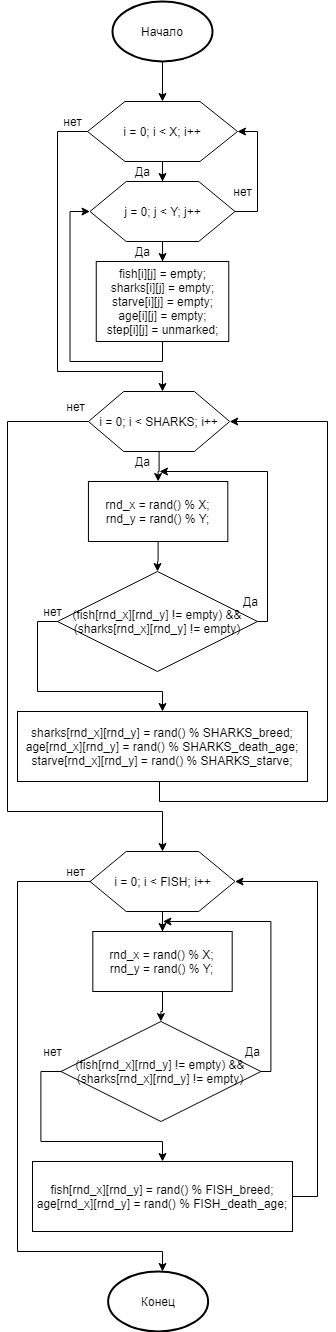
\includegraphics[width=0.3\textwidth]{initialization22.png}
  \caption{Подпрограмма initialization\label{first}}
\end{figure}
\newpage
\begin{figure}[!h]
  \centering
  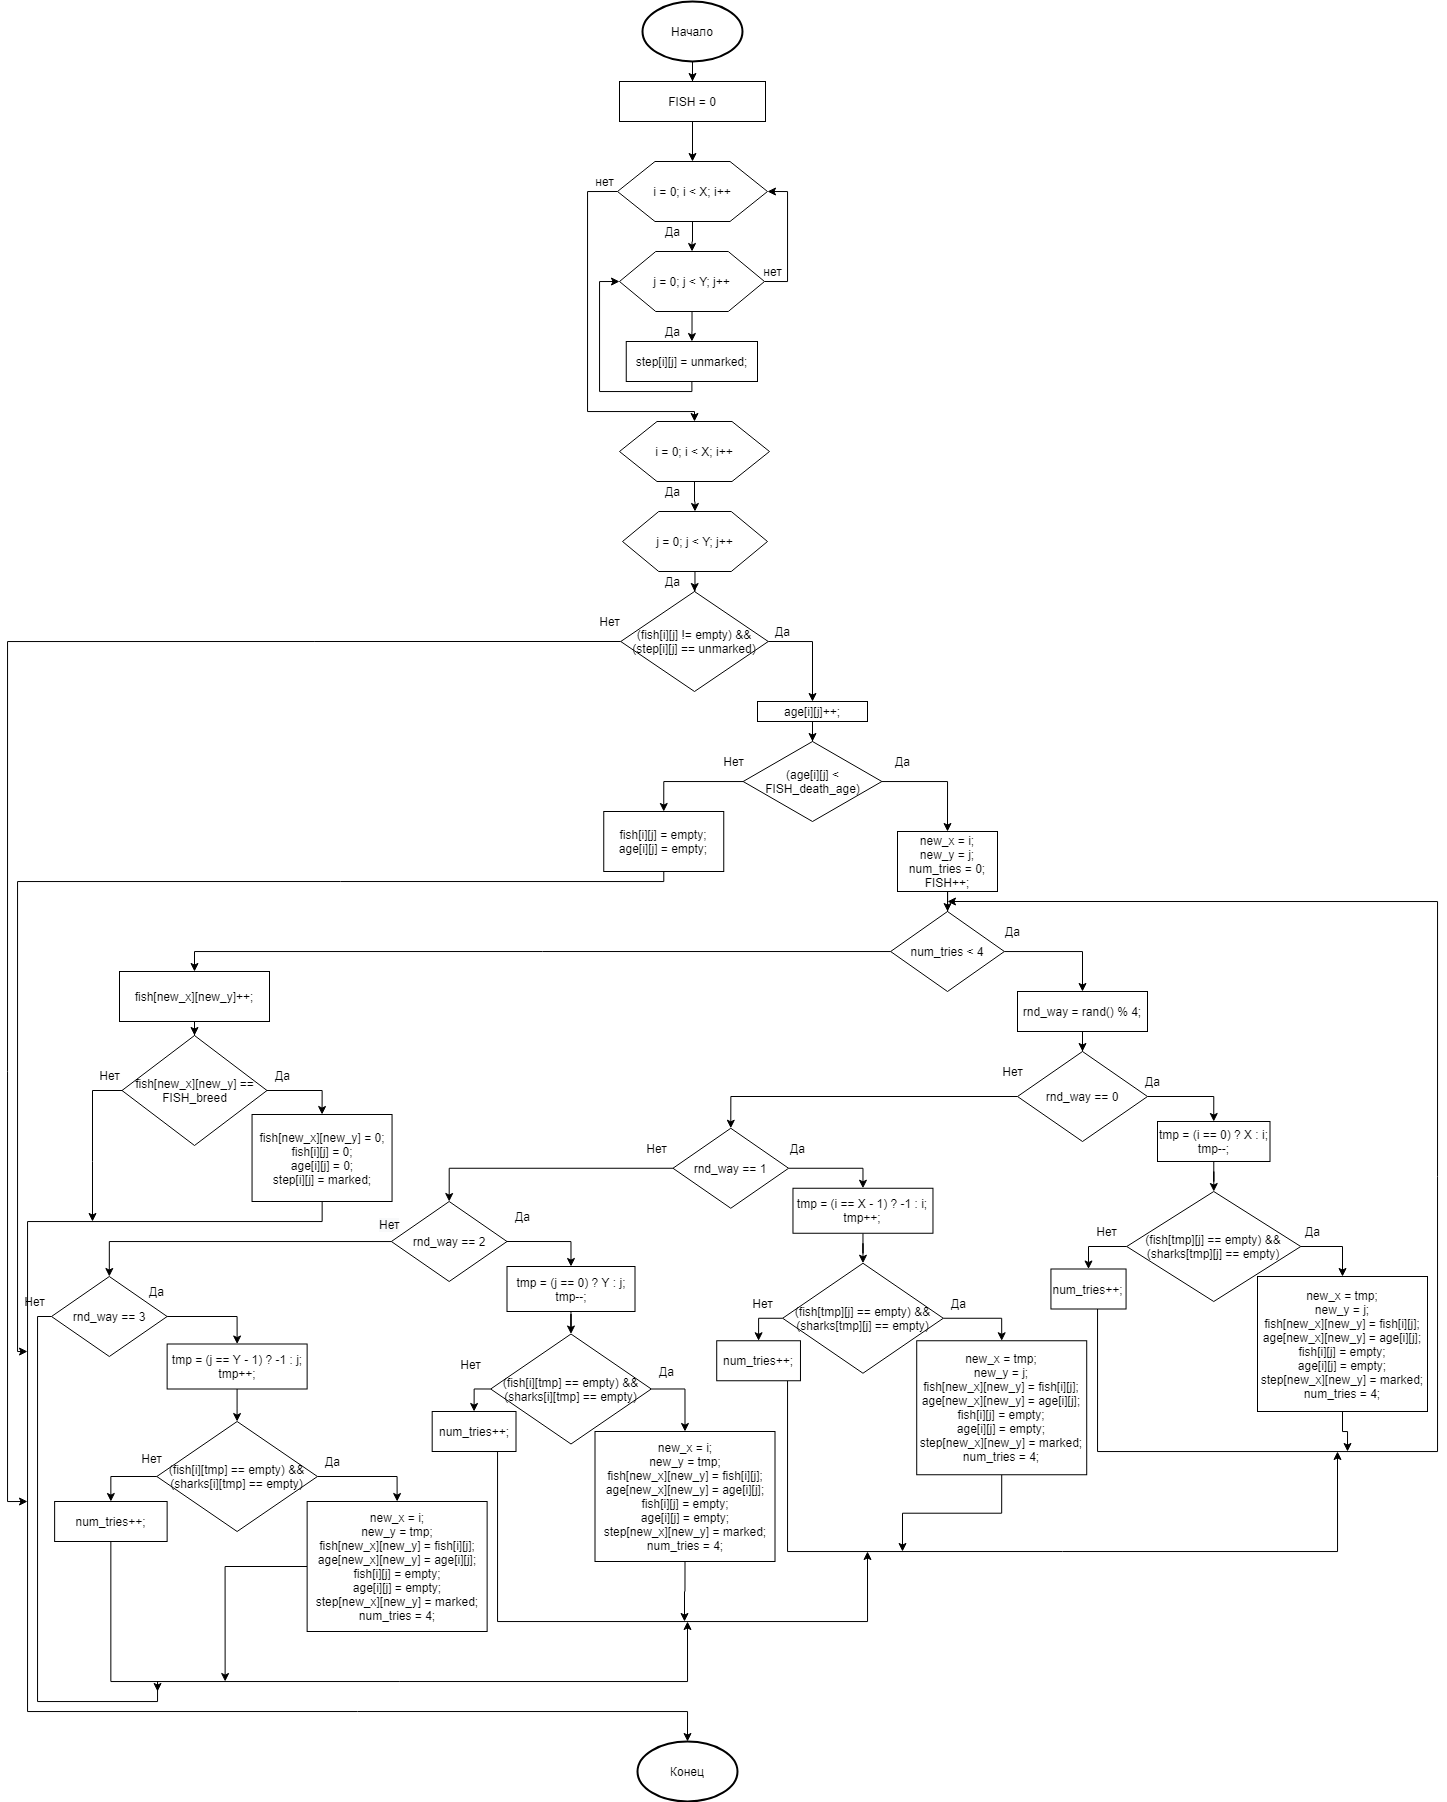
\includegraphics[width=1\textwidth]{fishstep.png}
  \caption{Подпрограмма Fishstep\label{second}}
\end{figure}
\newpage
\begin{figure}[!h]
  \centering
  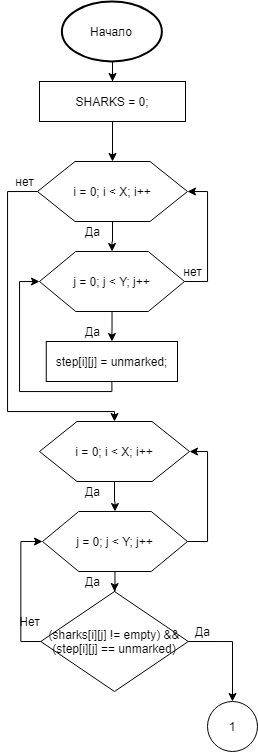
\includegraphics[width=0.3\textwidth]{sharkstepTEST2.png}
  \caption{Подпрограмма Sharkstep\label{second}}
\end{figure}
\newpage
\begin{figure}[!h]
  \centering
  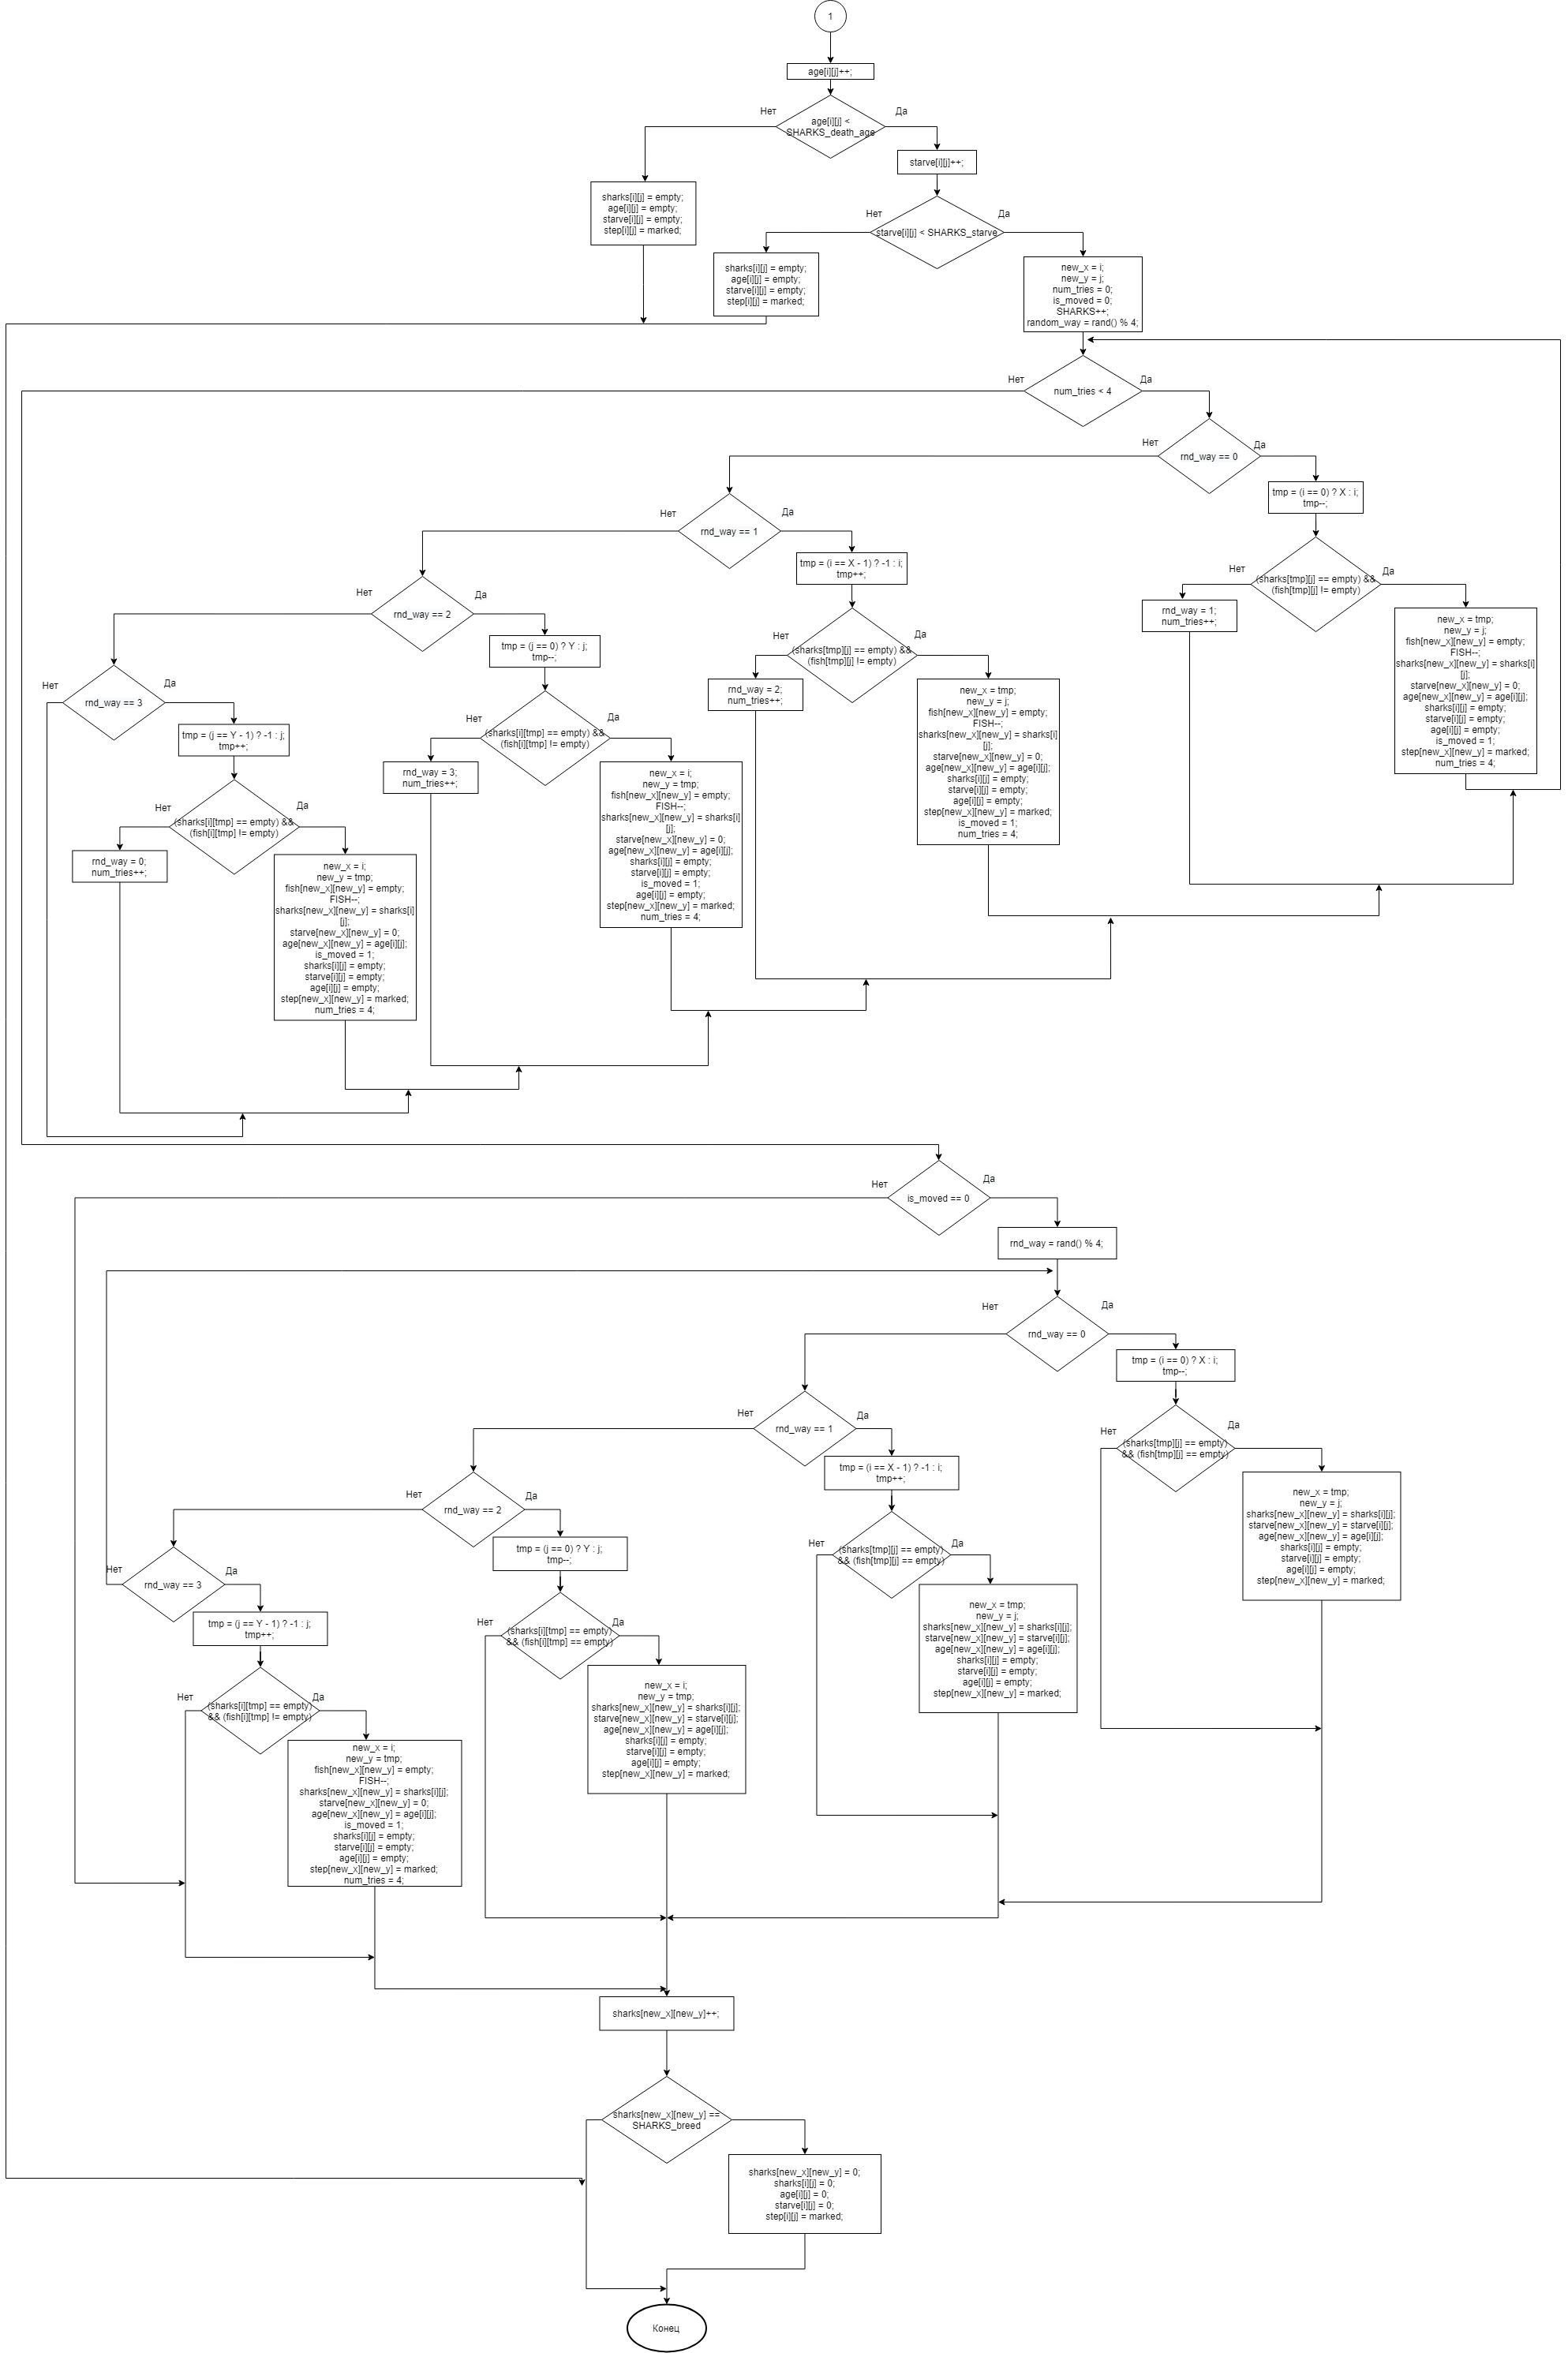
\includegraphics[width=0.8\textwidth]{sharkstepTEST.png}
  \caption{Подпрограмма Sharkstep\label{second}}
\end{figure}


\newpage
\begin{figure}[!h]
  \centering
  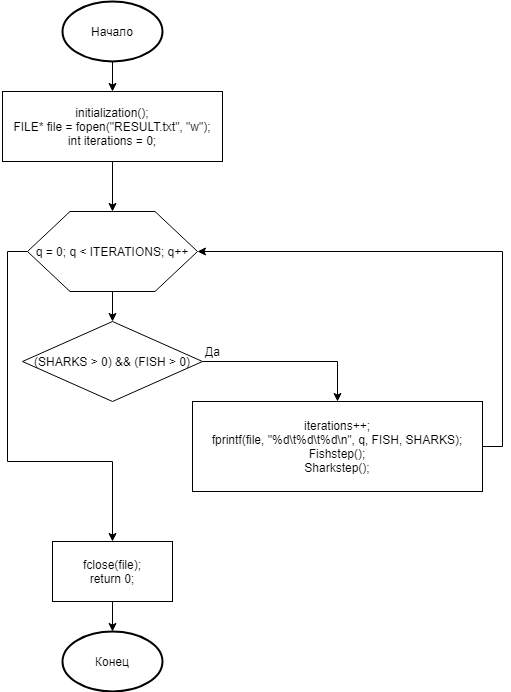
\includegraphics[width=0.6\textwidth]{main.png}
  \caption{Подпрограмма main\label{second}}
\end{figure}

\newpage
Зависимость численности акул и рыб от времени получилась следующая.
\begin{figure}[!h]
  \centering
  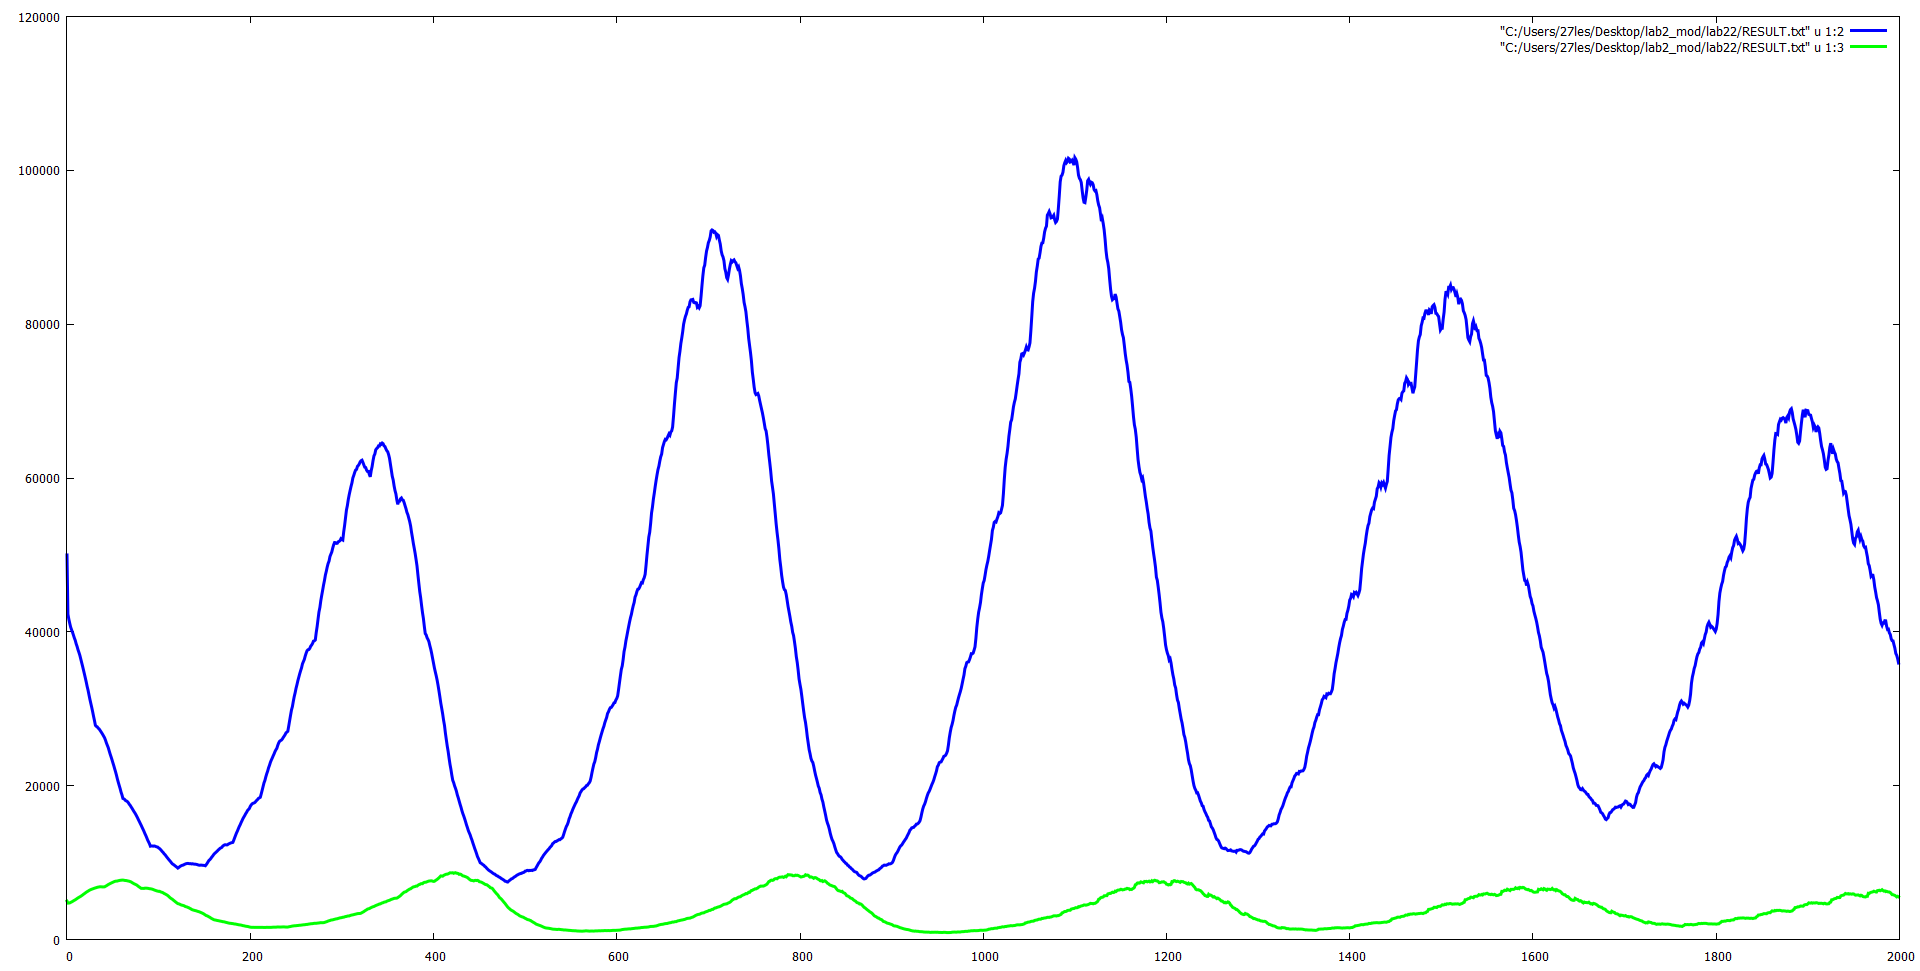
\includegraphics[width=1\textwidth]{RESULT.png}
  \caption{Синие - рыбы, зеленые - акулы\label{second}}
\end{figure}



\addcontentsline{toc}{section}{Приложение}
\section*{Приложение}
\begin{minted}[mathescape,linenos,frame=lines]{C}
#include <iostream>
#include <stdio.h>
#include <stdlib.h>
#include <time.h>
#define ITERATIONS 2000 
#define X 500 
#define Y 500
int FISH = 50000; 
int SHARKS = 5000; 
int FISH_breed = 30; 
int SHARKS_breed = 40; 
int SHARKS_starve = 25; 
int FISH_death_age = 100;
int SHARKS_death_age = 200;
int step[X][Y]; 
int fish[X][Y]; 
int sharks[X][Y]; 
int starve[X][Y]; 
int age[X][Y]; 
int i, j;
enum { empty = -1, marked, unmarked };
void initialization()
{
int random_x, random_y;
for (i = 0; i < X; i++) {
for (j = 0; j < Y; j++) {
fish[i][j] = empty;
sharks[i][j] = empty;
starve[i][j] = empty;
age[i][j] = empty;
step[i][j] = unmarked;
}
}
for (i = 0; i < SHARKS; i++) {
do {
random_x = rand() % X;
random_y = rand() % Y;
} while ((fish[random_x][random_y] != empty) &&
(sharks[random_x][random_y] != empty));
sharks[random_x][random_y] = rand() % SHARKS_breed;
age[random_x][random_y] = rand() % SHARKS_death_age;
starve[random_x][random_y] = rand() % SHARKS_starve;
}
for (i = 0; i < FISH; i++) {
do {
random_x = rand() % X;
random_y = rand() % Y;
} while ((fish[random_x][random_y] != empty) && 
(sharks[random_x][random_y] != empty));
fish[random_x][random_y] = rand() % FISH_breed;
age[random_x][random_y] = rand() % FISH_death_age;
}
}
void Fishstep()
{
static int new_x, new_y;
static int random_way, num_tries, tmp;
FISH = 0;
for (i = 0; i < X; i++) {
for (j = 0; j < Y; j++) {
step[i][j] = unmarked;
}
}
for (i = 0; i < X; i++) {
for (j = 0; j < Y; j++) {
if ((fish[i][j] != empty) && (step[i][j] == unmarked)) {
age[i][j]++;
if ((age[i][j] < FISH_death_age)) {
new_x = i;
new_y = j;
num_tries = 0;
FISH++;
while (num_tries < 4) {
random_way = rand() % 4;
if (random_way == 0) {
tmp = (i == 0) ? X : i;
tmp--;
if ((fish[tmp][j] == empty) && (sharks[tmp][j] == empty)) {
new_x = tmp;
new_y = j;
fish[new_x][new_y] = fish[i][j];
age[new_x][new_y] = age[i][j];
fish[i][j] = empty;
age[i][j] = empty;
step[new_x][new_y] = marked;
num_tries = 4;
}
else {
num_tries++;
}
}
else if (random_way == 1) {
tmp = (i == X - 1) ? -1 : i;
tmp++;
if ((fish[tmp][j] == empty) && (sharks[tmp][j] == empty)) {
new_x = tmp;
new_y = j;
fish[new_x][new_y] = fish[i][j];
age[new_x][new_y] = age[i][j];
fish[i][j] = empty;
age[i][j] = empty;
step[new_x][new_y] = marked;
num_tries = 4;
}
else {
num_tries++;
}
}
else if (random_way == 2) {
tmp = (j == 0) ? Y : j;
tmp--;
if ((fish[i][tmp] == empty) && (sharks[i][tmp] == empty)) {
new_x = i;
new_y = tmp;
fish[new_x][new_y] = fish[i][j];
age[new_x][new_y] = age[i][j];
fish[i][j] = empty;
age[i][j] = empty;
step[new_x][new_y] = marked;
num_tries = 4;
}
else {
num_tries++;
}
}
else if (random_way == 3) {
tmp = (j == Y - 1) ? -1 : j;
tmp++;
if ((fish[i][tmp] == empty) && (sharks[i][tmp] == empty)) {
new_x = i;
new_y = tmp;
fish[new_x][new_y] = fish[i][j];
age[new_x][new_y] = age[i][j];
fish[i][j] = empty;
age[i][j] = empty;
step[new_x][new_y] = marked;
num_tries = 4;
}
else {
num_tries++;
}
}
}
fish[new_x][new_y]++;
if (fish[new_x][new_y] == FISH_breed) {
fish[new_x][new_y] = 0;
fish[i][j] = 0;
age[i][j] = 0;
step[i][j] = marked;
}
}
else {
fish[i][j] = empty;
age[i][j] = empty;
}
}
}
}
}
void Sharkstep()
{
static int new_x, new_y;
static int random_way, num_tries, tmp;
static int is_moved;
SHARKS = 0;
for (i = 0; i < X; i++) {
for (j = 0; j < Y; j++) {
step[i][j] = unmarked;
}
}
for (i = 0; i < X; i++) {
for (j = 0; j < Y; j++) {
if ((sharks[i][j] != empty) && (step[i][j] == unmarked)) {
age[i][j]++;
if (age[i][j] < SHARKS_death_age) {
starve[i][j]++;
if (starve[i][j] < SHARKS_starve) {
new_x = i;
new_y = j;
num_tries = 0;
is_moved = 0;
SHARKS++;
random_way = rand() % 4;
while (num_tries < 4) {
if (random_way == 0) {
tmp = (i == 0) ? X : i;
tmp--;
if ((sharks[tmp][j] == empty) && (fish[tmp][j] != empty)) {
new_x = tmp;
new_y = j;
fish[new_x][new_y] = empty;
FISH--;
sharks[new_x][new_y] = sharks[i][j];
starve[new_x][new_y] = 0;
age[new_x][new_y] = age[i][j];
sharks[i][j] = empty;
starve[i][j] = empty;
age[i][j] = empty;
is_moved = 1;
step[new_x][new_y] = marked;
num_tries = 4;
}
else {
random_way = 1;
num_tries++;
}
}
else if (random_way == 1) {
tmp = (i == X - 1) ? -1 : i;
tmp++;
if ((sharks[tmp][j] == empty) && (fish[tmp][j] != empty)) {
new_x = tmp;
new_y = j;
fish[new_x][new_y] = empty;
FISH--;
sharks[new_x][new_y] = sharks[i][j];
starve[new_x][new_y] = 0;
age[new_x][new_y] = age[i][j];
sharks[i][j] = empty;
starve[i][j] = empty;
age[i][j] = empty;
step[new_x][new_y] = marked;
is_moved = 1;
num_tries = 4;
}
else {
random_way = 2;
num_tries++;
}
}
else if (random_way == 2) {
tmp = (j == 0) ? Y : j;
tmp--;
if ((sharks[i][tmp] == empty) && (fish[i][tmp] != empty)) {
new_x = i;
new_y = tmp;
fish[new_x][new_y] = empty;
FISH--;
sharks[new_x][new_y] = sharks[i][j];
starve[new_x][new_y] = 0;
age[new_x][new_y] = age[i][j];
sharks[i][j] = empty;
starve[i][j] = empty;
is_moved = 1;
age[i][j] = empty;
step[new_x][new_y] = marked;
num_tries = 4;
}
else {
random_way = 3;
num_tries++;
}
}
else if (random_way == 3) {
tmp = (j == Y - 1) ? -1 : j;
tmp++;
if ((sharks[i][tmp] == empty) && (fish[i][tmp] != empty)) {
new_x = i;
new_y = tmp;
fish[new_x][new_y] = empty;
FISH--;
sharks[new_x][new_y] = sharks[i][j];
starve[new_x][new_y] = 0;
age[new_x][new_y] = age[i][j];
is_moved = 1;
sharks[i][j] = empty;
starve[i][j] = empty;
age[i][j] = empty;
step[new_x][new_y] = marked;
num_tries = 4;
}
else {
random_way = 0;
num_tries++;
}
}
}
if (is_moved == 0) {
random_way = rand() % 4;
if (random_way == 0) {
tmp = (i == 0) ? X : i;
tmp--;
if ((sharks[tmp][j] == empty) && (fish[tmp][j] == empty)) {
new_x = tmp;
new_y = j;
sharks[new_x][new_y] = sharks[i][j];
starve[new_x][new_y] = starve[i][j];
age[new_x][new_y] = age[i][j];
sharks[i][j] = empty;
starve[i][j] = empty;
age[i][j] = empty;
step[new_x][new_y] = marked;
}
}
else if (random_way == 1) {
tmp = (i == X - 1) ? -1 : i;
tmp++;
if ((sharks[tmp][j] == empty) && (fish[tmp][j] == empty)) {
new_x = tmp;
new_y = j;
sharks[new_x][new_y] = sharks[i][j];
starve[new_x][new_y] = starve[i][j];
age[new_x][new_y] = age[i][j];
sharks[i][j] = empty;
starve[i][j] = empty;
age[i][j] = empty;
step[new_x][new_y] = marked;
}
}
else if (random_way == 2) {
tmp = (j == 0) ? Y : j;
tmp--;
if ((sharks[i][tmp] == empty) && (fish[i][tmp] == empty)) {
new_x = i;
new_y = tmp;
sharks[new_x][new_y] = sharks[i][j];
starve[new_x][new_y] = starve[i][j];
age[new_x][new_y] = age[i][j];
sharks[i][j] = empty;
starve[i][j] = empty;
age[i][j] = empty;
step[new_x][new_y] = marked;
}
}
else if (random_way == 3) {
tmp = (j == Y - 1) ? -1 : j;
tmp++;
if ((sharks[i][tmp] == empty) && (fish[i][tmp] == empty)) {
new_x = i;
new_y = tmp;
sharks[new_x][new_y] = sharks[i][j];
starve[new_x][new_y] = starve[i][j];
age[new_x][new_y] = age[i][j];
sharks[i][j] = empty;
starve[i][j] = empty;
age[i][j] = empty;
step[new_x][new_y] = marked;
}
}
}
sharks[new_x][new_y]++;
if (sharks[new_x][new_y] == SHARKS_breed) {
sharks[new_x][new_y] = 0;
sharks[i][j] = 0;
age[i][j] = 0;
starve[i][j] = 0;
step[i][j] = marked;
}
}
else {
sharks[i][j] = empty;
age[i][j] = empty;
starve[i][j] = empty;
step[i][j] = marked;
}
}
else {
sharks[i][j] = empty;
age[i][j] = empty;
starve[i][j] = empty;
step[i][j] = marked;
}
}
}
}
}
int main(int argc, char** argv)
{
srand(time(NULL));
initialization();
printf("\nCalculating...\n");
FILE* file = fopen("RESULT.txt", "w");
int iterations = 0;
for (int q = 0; q < ITERATIONS; q++) {
if ((SHARKS > 0) && (FISH > 0)) {
iterations++;
fprintf(file, "%d\t%d\t%d\n", q, FISH, SHARKS);
Fishstep();
Sharkstep();
}
}
fclose(file);
return 0;
}
\end{minted}
\end{document}
